\documentclass[11pt,a4paper]{article}
\usepackage[margin=2.4cm]{geometry}
\usepackage{amsmath,amssymb,amsthm,bm}
\usepackage{booktabs,graphicx,xcolor,enumitem}
\usepackage[framemethod=default]{mdframed}
\usepackage[numbers]{natbib}
\usepackage[colorlinks=true,linkcolor=blue!50!black,citecolor=blue!50!black,urlcolor=blue!50!black]{hyperref}

\newcommand{\R}{\mathbb{R}}
\newcommand{\E}{\mathbb{E}}
\newcommand{\sg}{\operatorname{sg}}
\newcommand{\citeq}[1]{\textcolor{red!70!black}{[CITE?: #1]}}
\newcommand{\status}[1]{\textsf{\small[#1]}}
\newtheorem*{example}{Worked example}
\newmdenv[linecolor=black!30,backgroundcolor=black!3,innertopmargin=6pt,innerbottommargin=6pt]{keybox}
\newcommand{\misconception}[3]{\begin{keybox}\textbf{Misconception.} #1\par\smallskip
  \textbf{Where it fails.} #2\par\smallskip\textbf{What it over-generalises.} #3\end{keybox}}

\title{Structural losses for heavy rain:\\ the Minkowski loss, flow matching, and where the gradient goes}
\author{minkowski-loss project notes \quad (DECISIONS \S37--\S40)}
\date{30 October 2026}

\begin{document}
\sloppy
\maketitle

\noindent\textbf{What these notes are for.} They collect, in one place and from first principles, everything needed to
understand how the Minkowski loss acts on the two models of the project: the deterministic U-Net (Study~1) and the
flow-matching residual model (Study~2). Every loss is written out. Every claim carries a label:
\status{derivation} follows from the stated definitions; \status{measured} was run in this project (the file is
given); \status{inference} is our reading, not tested directly; \status{withdrawn} was claimed earlier and is wrong.
All numbers refer to the hourly v4 data (\texttt{patches\_v4\_adv}), the hourly vanilla backbone
\texttt{UNet\_Ana\_20261021\_211732} (last checkpoint) and the clean flow-matching model
\texttt{Extremes\_20261026\_092630/fm\_best.pth}, on validation subsets, with one training seed.

\tableofcontents

%=====================================================================
\section{The problem in one page}
%=====================================================================

We want 2-km precipitation fields from 12.5-km inputs that get \emph{heavy rain} right: how much of it there is, how
intense it gets and what shape it has. Two observations drive the whole project.

\begin{enumerate}[leftmargin=1.4em]
\item \textbf{Pixel losses do not care about heavy rain.} Pixels above 20\,mm are about $10^{-3}$ of the pixels of a
heavy patch and $10^{-4}$ of a random one. Any loss that averages over pixels gives them a tiny share of its
gradient, so a model trained on it can afford to get them wrong. Section~\ref{sec:fmloss} measures this for the
flow-matching loss: about 1\% of its gradient.
\item \textbf{Structural statistics see heavy rain directly.} The Minkowski functionals describe the set of pixels
above a threshold $u$ (its area, its perimeter, how many pieces it has) at many thresholds, including high ones. A
loss on them can, in principle, give the top of the distribution its own weight.
\end{enumerate}

\noindent The notes follow one question: \emph{does the Minkowski loss actually put gradient on heavy rain, and if not,
why not and how do we fix it?} The short answer, built up in the sections below:
\begin{itemize}[nosep]
\item In its original form the loss gives each threshold a pull proportional to the \emph{number of pixels near that
threshold}, so light rain still dominates, and thresholds the prediction never reaches give \emph{no} gradient at all
(Section~\ref{sec:heavy}).
\item The fix (\texttt{REWARD\_FORM: quantile\_mass}) reads the area curve along the intensity axis and reweights
perimeter and Euler by inverse pixel mass. It moves the share of gradient on pixels $\ge20$\,mm from 3.7\% to 40.9\%
on heavy patches (Section~\ref{sec:fix}).
\item The tail mismatch is not hidden by noise: every reward feature sees it at 1--3 times the member spread. What
blocked the original form was \emph{reach} (Section~\ref{sec:stability}).
\end{itemize}

%=====================================================================
\section{Fields, the two spaces, and the base models}
%=====================================================================

\subsection{Model space}
A precipitation field is a vector $f\in\R_{\ge 0}^N$ of hourly accumulations in mm, $N = 128^2 = 16{,}384$ pixels of
$2\times 2$\,km. Networks work in the \emph{model space}
\begin{equation}\label{eq:z}
  z = \frac{\log(1+f)}{c},\qquad f = e^{cz}-1,\qquad c = \log(1+613\ \text{mm}) = 6.42 ,
\end{equation}
so $z\in[0,1]$. Two identities return repeatedly: $\log(1+f) = cz$, and $\partial f/\partial z = c\,(1+f)$. The second
says that a small step in $z$ is a large step in mm for a heavy pixel: at $f = 50$\,mm, $\partial f/\partial z = 327$\,mm.

\subsection{The deterministic backbone and its loss (Study 1)}
A U-Net maps the coarse input $X$ to a prediction $\hat z = \mu_\theta(X)$. The vanilla loss is the pixel mean squared
error in model space,
\begin{equation}\label{eq:mse}
  \mathcal L_{\mathrm{MSE}}(\theta) = \frac1N\sum_{i=1}^{N}\big(\hat z_i - z_i\big)^2 .
\end{equation}

\paragraph{What it converges to.} \status{derivation} For one pixel, $\min_{a}\E[(a - Z)^2\mid X]$ is reached at
$a^\star = \E[Z\mid X]$, the conditional mean. Where the coarse input cannot tell where inside a 12.5-km cell the core
will be, the conditional mean spreads the core over all the places it could be.

\begin{example}
Suppose that, given $X$, a 2-km pixel has a 20\% chance of 50\,mm and an 80\% chance of 1\,mm. In model space,
$z = \log(51)/6.42 = 0.612$ or $\log 2/6.42 = 0.108$. The MSE optimum is $a^\star = 0.2\times0.612 + 0.8\times0.108 =
0.209$, i.e.\ $f = e^{6.42\times0.209} - 1 = 2.8$\,mm. The model predicts 2.8\,mm everywhere and never 50\,mm. The
mean in log space is a geometric-type mean, which falls even further below the 50\,mm peak than the arithmetic mean
(10.8\,mm) would.
\end{example}

\noindent This is the smoothing that the structural loss is meant to counteract in Study~1.

\paragraph{The structural loss in Study 1.} The deterministic objective is
\begin{equation}\label{eq:det}
  \mathcal L_{\mathrm{det}} = \mathcal L_{\mathrm{MSE}} + w(e)\; D_{\mathrm{Mink}}\big(f(\hat z),\, g^{\mathrm{obs}}\big),
\end{equation}
with $D_{\mathrm{Mink}}$ the distance of Section~\ref{sec:mink} summed over its three channels, and $w(e)$ a cosine
warm-up from 0 to $w_{\max}$ over the first epochs (\texttt{src/trainers/unet\_analytical.py}). Hourly data needed a new
$w_{\max}$ (DECISIONS \S37); Section~\ref{sec:study1} summarises the bracket.

\subsection{The flow-matching residual model (Study 2)}
Flow matching (FM) learns the part of the target the backbone cannot predict. With $\mu$ the backbone prediction and
$Y$ the target in model space, the \emph{residual} is
\begin{equation}
  r = \frac{Y-\mu}{\sigma_r},\qquad \sigma_r = 0.01267 \quad\text{(hourly vanilla backbone, train split)},
\end{equation}
scaled to be roughly unit size. FM learns a velocity field $v_\theta(x,t,\mathbf c)$, condition $\mathbf c = [X,\mu]$,
that carries Gaussian noise $x_0$ at $t=0$ to residuals at $t=1$. Training draws $x_0\sim\mathcal N(0,I)$,
$t\sim U(0,1)$, forms the straight path $x_t = (1-t)x_0 + t\,r$ and regresses the velocity of that path:
\begin{equation}\label{eq:fm}
  \mathcal L_{\mathrm{FM}}(\theta) = \E_{t,x_0,(r,\mathbf c)}\;\frac1N\big\| v_\theta(x_t,t,\mathbf c) - (r - x_0)\big\|^2 .
\end{equation}

\paragraph{What it converges to, and why that differs from the backbone.} \status{derivation} Again an MSE, so the
optimum is a conditional mean, but now of the \emph{path velocity given the current state}:
$v^\star(x,t,\mathbf c) = \E[r - x_0\mid x_t = x,\mathbf c]$. Integrating $\mathrm dx/\mathrm dt = v^\star$ from noise
transports the noise distribution exactly onto $p(r\mid\mathbf c)$ \citeq{flow matching / rectified flow, marginal
velocity theorem}. So the FM loss is \emph{not} biased toward the mean in principle: at its optimum the sampler
reproduces the whole conditional distribution, tail included. The bias toward the mean in the backbone comes from
asking for one field; FM asks for a velocity at every intermediate state, which is a different question.

\paragraph{What goes wrong in practice.} The optimum is not reached. With a finite network and finite training, the
error ends up where the loss is least sensitive. Equation~\eqref{eq:fm} is a pixel mean, so heavy pixels are a
tiny part of it. Section~\ref{sec:fmloss} measures how tiny. The clean hourly FM produces about 3 in 10 of the observed
exceedances of 50.1\,mm on heavy patches (Table~\ref{tab:fm}).

\paragraph{Sampling.} Heun's method, 16 steps of $h = 1/16$:
\begin{equation}\label{eq:heun}
  x_{k+1} = x_k + \tfrac h2\Big[v_\theta(x_k,t_k) + v_\theta\big(x_k + h\,v_\theta(x_k,t_k),\,t_k+h\big)\Big],
\end{equation}
and the generated field is $f = e^{c\,\mathrm{clamp}(\mu + \sigma_r x_{16},\,0,\,1)}-1$.

%=====================================================================
\section{The Minkowski functionals and the structural distance}\label{sec:mink}
%=====================================================================

\paragraph{What is measured.} For a threshold $u$, the \emph{excursion set} is $E_u = \{i : f_i \ge u\}$. Three numbers
describe its geometry: its area $A(u)$, its perimeter $P(u)$ and its Euler characteristic $\chi(u)$ (number of pieces
minus number of holes). In two dimensions these are, up to linear combination, the only additive, continuous,
motion-invariant functionals of a set \citeq{Hadwiger's characterisation theorem}. The loss uses $Q = 15$ thresholds,
evenly spaced in $\xi = \log u$:
\[
u \in \{0.1,\, 0.192,\, 0.314,\, 0.509,\, 0.828,\, 1.35,\, 2.11,\, 3.43,\, 5.36,\, 8.61,\, 13.5,\, 20.2,\, 31.7,\, 50.1,\, 79.0\}\,\text{mm}.
\]

\paragraph{Discrete, differentiable estimators} (\texttt{src/losses/minkowski.py}). The hard indicator
$\mathbb 1[f_i\ge u]$ has zero derivative almost everywhere. The loss therefore uses a \emph{soft mask}
\begin{equation}\label{eq:mask}
  s_i(u) = \sigma\!\left(\frac{f_i-u}{\tau_u}\right),\qquad \tau_u = \max(0.1\, a\, u,\ 10^{-3}),
\end{equation}
with $\sigma$ the logistic function and anneal factor $a$; at $a = 0.05$ (the reward), $\tau_u = 0.005\,u$, which is
0.25\,mm at $u = 50$\,mm. Then
\begin{align}
  A(u) &= \ell^2\sum_i \mathbb 1[f_i\ge u]\ \ \text{(forward)},\qquad
         \frac{\partial A}{\partial f_i} := \ell^2\,\frac{\partial s_i}{\partial f_i}\ \ \text{(backward)},\\
  P(u) &= \ell\Big[w_{\mathrm{ax}}\!\!\sum_{\text{axial pairs}}\!|s_i-s_j| + w_{\mathrm{di}}\!\!\sum_{\text{diagonal pairs}}\!|s_i-s_j|\Big],\\
  \chi(u) &= V - E_x - E_y + F ,
\end{align}
with $\ell = 2$\,km, Cauchy--Crofton weights $w_{\mathrm{ax}} = 0.473$, $w_{\mathrm{di}} = 0.218$, and $V,E,F$ soft counts
of pixels, edges and faces (an edge or face counts with the minimum of its pixels' masks). The area uses a
\emph{straight-through estimator}: the exact count in the forward pass, the soft-mask derivative in the backward pass.

\paragraph{The curves and the distance.} Each field becomes three curves over the 15 thresholds,
\begin{equation}
  g(f) = \big[\log(1+A),\ \log(1+P),\ \operatorname{sign}(\chi)\log(1+|\chi|)\big] \in \R^{3\times 15},
\end{equation}
and two curves are compared by integrating the absolute difference over log-intensity,
\begin{equation}\label{eq:dist}
  d(g,h) = \frac13\sum_{k=1}^{3}\frac{1}{\xi_{15}-\xi_1}\int_{\xi_1}^{\xi_{15}} w_k(\xi)\,\big|g_k(\xi)-h_k(\xi)\big|\,\mathrm d\xi ,
\end{equation}
evaluated by the trapezoid rule on the thresholds, with weights $w_k\equiv1$ in the original form (Section~\ref{sec:fix}
introduces other weights). The deterministic loss \eqref{eq:det} uses the channel \emph{sum}, $D_{\mathrm{Mink}} = 3d$;
the reward uses the channel mean $d$. Every decade of intensity gets equal weight \emph{in this sum}.
Section~\ref{sec:heavy} shows why that is not equal weight in the gradient.

\paragraph{What the functionals cannot see.} They do not change when the field is shifted or rotated. A loss on them
cannot tell the model \emph{where} rain falls; that must come from a pixel-aligned term (the MSE, or the FM loss).
This is why no Minkowski variant improves FSS at the 1-pixel scale.

\subsection{Study 1 on hourly data, in brief}\label{sec:study1}
\status{measured, DECISIONS \S37} Bracket of $w_{\max}$, validation, last checkpoints, $u = 50.1$\,mm:

\begin{center}\small\begin{tabular}{lcccc}\toprule
$w_{\max}$ & $\Delta$MAE & exceedance ratio & RL bias $\lambda$10 / 100 / 1000 & FSS 50.1\,mm 1 / 21 px\\\midrule
0 (vanilla) & 0 & 0.113 & $-44$ / $-31$ / $-13$\% & 0.106 / 0.383\\
$6.0\times10^{-5}$ & +4.7\% & 0.192 & $-37$ / $-41$ / $-44$\% & 0.097 / 0.417\\
$1.8\times10^{-4}$ & +7.9\% & 0.287 & $-32$ / $-36$ / $-41$\% & 0.118 / 0.535\\
$5.4\times10^{-4}$ & +12.5\% & 0.442 & $-25$ / $-32$ / $-39$\% & 0.131 / 0.648\\
$1.8\times10^{-3}$ & +19.0\% & 0.607 & $-18$ / $-21$ / $-24$\% & 0.125 / 0.714\\\bottomrule
\end{tabular}\end{center}

\noindent More weight gives more exceedances, higher peaks and better FSS at 21\,px, at a rising cost in MAE and,
visibly in the images, grid-aligned striping from $1.8\times10^{-4}$ upward. Only $6\times10^{-5}$ is inside the +5\% MAE
cap. Every Minkowski run under-predicts the long return levels more than vanilla does. The Study-1 weight on hourly
data is still open. All these runs use the \emph{original} threshold form, so everything in Section~\ref{sec:heavy}
applies to them too.

%=====================================================================
\section{How the Minkowski loss is coupled to flow matching}\label{sec:coupling}
%=====================================================================

\paragraph{Why it cannot simply be added.} The FM loss \eqref{eq:fm} lives on noisy intermediate states $x_t$, which are
not precipitation fields. The functionals only make sense on a finished field. The fine-tune therefore treats the
structural distance as a \emph{reward} on generated samples, following DRaFT-K \citep{clark2024draft}: generate a
sample, score it, and back-propagate the score through the sampler into $\theta$.

\paragraph{DRaFT-K with $K=1$.} Back-propagating through all 16 Heun steps would store 32 network evaluations and spread
the credit thinly over the path. DRaFT-K cuts the graph: the first $16-K$ steps run with gradients off. With $K = 1$,
\begin{equation}
  x_{15} = \sg\big(\text{15 Heun steps from } x_0\big),\qquad x_{16} = \Phi_\theta(x_{15}),\qquad
  \nabla_\theta R = \frac{\partial R}{\partial x_{16}}\;\frac{\partial \Phi_\theta(x_{15})}{\partial\theta},
\end{equation}
where $\sg$ stops the gradient and $\Phi_\theta$ is the last Heun step \eqref{eq:heun}. Only the last $1/16$ of the
path is trained by the reward. \status{inference} In FM the last step mostly sets fine detail and amplitude, so a
$K=1$ reward acts on the smallest scales. The $K=1$ and $K=2$ gradients are aligned (cosine $+0.97$, \status{measured},
\texttt{logs/coupling\_v4adv\_*.log}), so $K=1$ is not missing a direction that $K=2$ would see.

\paragraph{One optimiser step.} For a batch of $B = 8$ conditions, draw $M$ members per condition, decode each to mm,
compute $g$ for each member, compare with the target curve $g^{\mathrm{obs}}$. The total fine-tune loss is
\begin{equation}\label{eq:total}
  L = w_{\mathrm r}\,R + w_{\mathrm p}\,\mathcal L_{\mathrm{prox}} + w_{\mathrm{ret}}\,\mathcal L_{\mathrm{FM}},
\end{equation}
optimised with AdamW, learning rate $10^{-5}$, gradient clipping at norm 1, 10 epochs of 500 steps.

\begin{table}[h]\centering\small
\begin{tabular}{lcc}\toprule
 & FM + dist & FM + energy\\\midrule
reward $R$ & distributional \eqref{eq:dist-reward} & energy score \eqref{eq:energy}\\
members $M$ & 4 & 16\\
$w_{\mathrm r}\ /\ w_{\mathrm p}\ /\ w_{\mathrm{ret}}$ & $10^{-3}$ / 1 / \textbf{0} & $10^{-3}$ / 1 / \textbf{1}\\
spread weight $\lambda_s$ & 0.5 & (not used)\\\bottomrule
\end{tabular}
\caption{The two hourly fine-tunes (startup lines of \texttt{logs/finetune\_v4adv\_\{dist,energy\}.log}; both start from
the clean FM, both use \texttt{config FM\_RESIDUAL\_SCALE=0.01267}).}
\end{table}

\paragraph{Where the mean and the MSE meet.} A common question is how the FM ``MSE'' and the Minkowski term interact.
In the distributional run they are \emph{not added}: $w_{\mathrm{ret}} = 0$. The MSE acts in three indirect ways. (1) It
produced the starting model. (2) The proximal anchor (below) is itself an MSE between the fine-tuned and the frozen
velocity field, a limit on how far the model may move, not a data term. (3) In the energy run it is present as the
retention term, and there, as Section~\ref{sec:budget} shows, it dominates.

\subsection{The distributional reward}
\begin{equation}\label{eq:dist-reward}
  R_{\mathrm{dist}} = \frac1B\sum_{b} d\Big(\tfrac1M\textstyle\sum_m g_{bm},\ g^{\mathrm{obs}}_b\Big)
  + \lambda_s\, d\Big(\log\!\big(1+\operatorname{std}_{b,m}\, g_{bm}\big),\ \log\!\big(1+\operatorname{std}_b\, g^{\mathrm{obs}}_b\big)\Big).
\end{equation}
The first term asks the \emph{average} member curve of each condition to match the observation. The second asks the
spread of the curves to match the spread of the observed curves.

\paragraph{What the spread term actually measures.} \status{derivation} Both standard deviations are pooled over the
batch: $\operatorname{std}_{b,m}$ runs over all $M\times B = 32$ generated curves. By the law of total variance,
\begin{equation}
  \operatorname{Var}_{b,m}(g) = \underbrace{\E_b\big[\operatorname{Var}_m(g\mid b)\big]}_{\text{ensemble spread}}
  + \underbrace{\operatorname{Var}_b\big(\E_m[g\mid b]\big)}_{\text{differences between patches}} .
\end{equation}
Eight different patches differ far more than four members of one patch do, so the second term dominates. As written,
the spread term mostly asks the eight patches to differ as much as their targets do. It does little to control the
ensemble's own spread. $R_{\mathrm{dist}}$ is \emph{not} a proper scoring rule (next subsection): a model can lower it
without matching the true conditional distribution.

\subsection{The energy reward}
\begin{equation}\label{eq:energy}
  R_{\mathrm{ES}} = \frac1B\sum_b\Big[\frac1M\sum_m d\big(g_{bm}, g^{\mathrm{obs}}_b\big)
   - \frac{1}{2M(M-1)}\sum_{m\ne m'} d\big(g_{bm}, g_{bm'}\big)\Big].
\end{equation}
The first term pulls every member toward the observation; the second rewards members that differ from each other.
This is an unbiased estimate of the \emph{energy score}
$\mathrm{ES}(P, y) = \E_P\, d(G, y) - \tfrac12\E_P\, d(G, G')$, with $G, G'$ independent draws from the model
\citeq{Gneiting \& Raftery 2007, energy score}.

\paragraph{Why $M(M-1)$ and not $M^2$.} \status{derivation} For independent members,
$\E\big[\frac{1}{M(M-1)}\sum_{m\ne m'} d(G_m,G_{m'})\big] = \E\, d(G,G')$. Dividing the same sum by $M^2$ gives
$\frac{M-1}{M}\E\,d(G,G')$: the bonus for spread shrinks, and the minimiser is an ensemble that is too narrow, which is
the failure the reward is meant to correct.

\paragraph{Proper scores.} A scoring rule is \emph{proper} if its expected value is smallest when the model's
distribution equals the true one. For a distance $d$ of negative type, the energy score is proper: the gap between
using $P$ and the truth $Q$ is half the energy distance between them, which is non-negative. The trapezoid integral
\eqref{eq:dist} is a weighted $L^1$ distance between 45-dimensional vectors, and $L^1$ distances are of negative type,
so $R_{\mathrm{ES}}$ is proper for the distribution of the curves $g$ \status{derivation, given the negative-type
property}. Whether it is \emph{strictly} proper (the truth is the unique minimiser) with an $L^1$ distance, we do not
know \citeq{strong negative type of $\ell^1$ metrics}. And proper only ever means proper \emph{on the features}: two
field distributions with the same distribution of curves score the same.

\subsection{The proximal anchor and the retention term}
\begin{equation}
  \mathcal L_{\mathrm{prox}} = \big\|v_\theta(\tilde x_t, t,\mathbf c) - v_{\mathrm{ref}}(\tilde x_t,t,\mathbf c)\big\|^2,
  \qquad \tilde x_t = (1-t)\,x_0 + t\,\tilde x_1,
\end{equation}
where $v_{\mathrm{ref}}$ is the frozen clean model. It should keep the fine-tuned velocity close to the clean one where
the sampler goes. The retention term is the FM loss \eqref{eq:fm} on the true residual; it is the only pixel-aligned
data term available, since the reward cannot see position.

\paragraph{The anchor is evaluated where the sampler never goes.} \status{derivation from the code,
\texttt{reward\_finetune.py}, the \texttt{x1 = ...} line} The code sets $\tilde x_1 = \mathrm{clamp}(f/6.42,\,0,\,1)$: the
generated field \emph{in mm}, divided by $c$ and saturating at 6.4\,mm. The model's coordinate is the scaled
log-residual $r = (Y-\mu)/\sigma_r$, mostly near 0 and of order $\pm1$, with outliers to $|r|\approx 34$.
\begin{example}
A pixel with 10\,mm gives $\tilde x_1 = \min(10/6.42, 1) = 1$ wherever it is. A residual of $0.05$ in model space (the
backbone 0.05 below the target, a factor $e^{0.05c}\approx1.38$ in $1+f$) is $r = 0.05/0.01267 \approx 3.9$.
\end{example}
\noindent So $\tilde x_t$ blends noise with a binary-looking rain mask, states the ODE does not visit, and the anchor
constrains the velocity there. In the dist run, which has no retention term, this anchor is the only thing holding the
model near the clean one. This must be fixed before any new fine-tune (Section~\ref{sec:plan}).

%=====================================================================
\section{How the terms share the update: the gradient budget}\label{sec:budget}
%=====================================================================

\paragraph{Weights are not what matters; gradient mix is.} \status{derivation} Adam's update is
$\Delta\theta = -\eta\,\hat m/(\sqrt{\hat v}+\epsilon)$, with $\hat m,\hat v$ running averages of the gradient and its
square. Multiplying every gradient by a constant $\lambda$ multiplies $\hat m$ by $\lambda$ and $\sqrt{\hat v}$ by
$|\lambda|$, so the step is unchanged (while $\epsilon$ is negligible). Two consequences:
\begin{itemize}[nosep]
\item A loss whose total gradient is tiny (the dist run: norm $8\times10^{-4}$, far below the clip at 1) still makes
full-size steps, all in its own direction.
\item When terms are added, what decides the direction is the \emph{ratio} of their gradients, not the weights.
$w_{\mathrm r} = 10^{-3}$ means nothing until it is compared with the other terms' gradient norms.
\end{itemize}

\paragraph{Measured at the clean checkpoint} (\texttt{scripts/evaluate/grad\_norm\_terms.py},
\texttt{logs/grad\_norm\_terms\_v4adv.txt}, four training batches) \status{measured}:
\begin{center}\small\begin{tabular}{lccccc}\toprule
run & reward & anchor & FM retention & reward share & $\cos(\nabla R,\nabla L)$\\\midrule
energy, original form & $8.3\times10^{-4}$ & $1.2\times10^{-4}$ & $0.65$ & 0.13\% & $-0.01$\\
dist, original form & $8.3\times10^{-4}$ & $0.7\times10^{-4}$ & 0 & 99\% & $+0.99$\\
energy, quantile\_mass & $5.0\times10^{-4}$ & & $0.65$ & 0.07\% & $-0.03$\\
dist, quantile\_mass & $5.0\times10^{-4}$ & & 0 & 96\% & $+0.97$\\\bottomrule
\end{tabular}\\[2pt]
{\footnotesize Norms of $\nabla_\theta$ of $w_{\mathrm r}R$, $w_{\mathrm p}\mathcal L_{\mathrm{prox}}$, $w_{\mathrm{ret}}\mathcal L_{\mathrm{FM}}$
before clipping; share $=\|\nabla(w_{\mathrm r}R)\|/\|\nabla L\|$.}
\end{center}

\noindent In the energy configuration the reward is 0.1\% of the gradient and orthogonal to the total. The energy
fine-tune is therefore, to a good approximation, more FM training at a low learning rate. Matching the reward's
gradient to the retention term's (the gradient-norm rule, DECISIONS \S9) means raising $w_{\mathrm r}$ by about three
orders of magnitude.

\subsection{What the two fine-tunes did}\label{sec:results}
\status{measured, DECISIONS \S38} 16 members, heun-16, $u = 50.1$\,mm, \texttt{fm\_mink\_latest.pth}. The clean FM was
evaluated twice (the evaluation does not seed its noise), which gives a crude noise level.

\begin{table}[h]\centering\small\resizebox{\linewidth}{!}{%
\begin{tabular}{lccc}\toprule
heavy subset (1,024 patches) & FM draws 1 / 2 & FM + dist & FM + energy\\\midrule
exceedances (of 1,537 observed) & 458 / 393 & \textbf{580} & 411\\
RL bias $\lambda$10 / 100 / 1000 & $-30/-36/-44$ ; $-33/-36/-36$\% & $\mathbf{-23/-20/-15}$\% & $-31/-33/-33$\%\\
FSS 31.7\,mm, 21 px & 0.707 / 0.707 & \textbf{0.741} & 0.726\\
FSS 50.1\,mm, 1 / 21 px & 0.114/0.506 ; 0.103/0.523 & 0.109 / \textbf{0.554} & 0.086 / 0.469\\
RAPSD distance & 1.14 / 1.19 & \textbf{0.81} & 1.24\\
anisotropy & 1.31 / 1.27 & 1.30 & 1.28\\
CRPS & 0.1613 / 0.1614 & 0.1598 & 0.1615\\\midrule
random subset (4,096): exceedance ratio & 0.272 & \textbf{0.517} & 0.228\\
\phantom{random subset (4,096):} RAPSD distance & 0.86 & \textbf{0.35} & 0.97\\\bottomrule
\end{tabular}}
\caption{Clean FM and its two fine-tunes on hourly data. One seed per model.}\label{tab:fm}
\end{table}

\begin{itemize}[leftmargin=1.2em]
\item \textbf{FM + dist} beats clean FM by more than the evaluation noise on the 100- and 1000-year return levels, FSS
at 31.7\,mm, the spectrum and CRPS; on the exceedance count by about 3 noise standard deviations. Yet its training
reward barely moved ($0.351\to0.339$), and its gradient was mostly on light rain. Why it helped the tail is not
established; Section~\ref{sec:fmloss} offers a candidate.
\item \textbf{FM + energy} sits inside the spread of the two clean-FM draws on every tail column and is slightly worse on
FSS at 50.1\,mm and on the spectrum. Its reward did not move ($0.199\to0.205$). Given the budget table this is expected:
the run tested nothing about the reward. Its one gain, FSS at 31.7\,mm, cannot be separated from the 5,000 extra FM
steps without the $w_{\mathrm r} = 0$ control. (Its GPD shape error is the best of the table, 0.011, next to a weak
tail: shape and scale trade off, which is why the shape column is not used to rank.)
\end{itemize}

%=====================================================================
\section{Why the original reward misses heavy rain}\label{sec:heavy}
%=====================================================================

\paragraph{One pixel, one threshold.} \status{derivation} Through the soft mask \eqref{eq:mask}, pixel $i$ feels
threshold $u$ only through
\begin{equation}\label{eq:sens}
  \frac{\partial s_i}{\partial f_i} = \frac{1}{\tau_u}\,\sigma'\!\left(\frac{f_i-u}{\tau_u}\right),\qquad
  \sigma'(a) = \sigma(a)\big(1-\sigma(a)\big)\approx e^{-|a|}\ \text{for}\ |a|\gg 1 .
\end{equation}
The kernel has width $\tau_u = 0.005u$: a pixel feels only the thresholds within a few per cent of its own value.

\begin{example}
A predicted core of 17\,mm under a target that exceeds 20.2, 31.7 and 50.1\,mm. For $u = 20.2$\,mm, $\tau = 0.101$\,mm and
$a = (17-20.2)/0.101 = -31.7$, so $\partial s/\partial f \approx e^{-31.7}/0.101 \approx 1.7\times10^{-13}$\,mm$^{-1}$.
For $u = 50.1$, $a = -132$ and $e^{-132}\approx 5\times10^{-58}$, which underflows to zero in single precision. The
thresholds where the error is largest are the ones that give no gradient. We call this the \textbf{reach} problem.
\end{example}

\paragraph{All pixels, one threshold: the pixel-mass limit.} \status{derivation} Summing \eqref{eq:sens} over pixels and
writing $p$ for the density of pixel values,
\begin{equation}
  \sum_i \frac{\partial s_i}{\partial f_i} = N\!\int p(f)\,\frac{1}{\tau}\sigma'\!\Big(\frac{f-u}{\tau}\Big)\mathrm df
  \;\longrightarrow\; N\,p(u)\quad (\tau\to0),
\end{equation}
because $\tau^{-1}\sigma'(\cdot/\tau)$ is a probability density of width $\sim\tau$ (it integrates to 1). A threshold's
total pull is the number of pixels per mm at $u$, \emph{whatever $\tau$ is}. Two results follow.
\begin{itemize}[nosep]
\item Light rain has most pixels, so it takes most of the gradient: on the clean hourly FM, 73\% of
$|\partial R/\partial z|$ lands on pixels below 1\,mm on the heavy subset, 89\% on the random subset, and 3.7\% /
0.2\% on pixels $\ge20$\,mm (Fig.~\ref{fig:share}) \status{measured}.
\item Changing the anneal factor changes $\tau$, so it cannot change the shares to leading order. This explains the
15-min sweep (DECISIONS \S5): anneal 0.05 $\to$ 0.40 raised the absolute tail gradient by eleven orders of magnitude
while the tail's share stayed at 0.75--0.88\%.
\end{itemize}

\misconception{``Equal weight per decade in the loss means equal weight per decade in training.''}
{The distance \eqref{eq:dist} weights decades equally, but the gradient of each decade's term is multiplied by the
number of pixels near it; above the prediction's maximum it is zero.}
{It is true for a quantity that is linear in the curve values. Here the curves' sensitivity to the field is itself
proportional to pixel mass.}

%=====================================================================
\section{The fix: quantile area and inverse-mass weights}\label{sec:fix}
%=====================================================================

The two failures need different fixes: (1) the gradient grows with pixel mass; (2) a threshold out of reach gives
nothing. Options considered, all keeping $K = 1$:
\begin{description}[leftmargin=1.2em,nosep]
\item[A. Inverse-mass weights.] Weight each threshold's term by $(n_j+1)^{-\alpha}$, $n_j$ the target's number of pixels
above $u_j$. Fixes (1), not (2).
\item[B. Hard forward, heavy-tailed backward.] Exact counts forward, a heavy-tailed kernel of width $\sim0.3u$
backward. Fixes (2), but adds a width hyperparameter, and a surrogate gradient can point where the true objective
does not, which is how gaming starts.
\item[C. Quantile form of the area.] Compare the area curve horizontally instead of vertically. Removes (2) exactly
for the area, with no new hyperparameter.
\end{description}
\noindent\textbf{Decision (researcher, 2026-10-29): C for the area, A for perimeter and Euler}
(\texttt{REWARD\_FORM: quantile\_mass}; the original stays as \texttt{REWARD\_FORM: threshold}, the default).

\subsection{The quantile area}
\paragraph{Same curve, read along the other axis.} The area curve is a \emph{survival function}:
$S_f(v) = \#\{i: f_i\ge v\}$, and $A(u) = \ell^2 S_f(u)$. Plot it with intensity horizontally and pixel count vertically
(Fig.~\ref{fig:survival}). The original loss compares the two curves \emph{vertically}: at a fixed intensity $u_j$, how
many pixels each field has above it. One can equally compare them \emph{horizontally}: at a fixed count $n$, which
intensity each field reaches. That intensity is the field's $n$-th largest value, $f_{(n)}$.

\begin{figure}[t]\centering
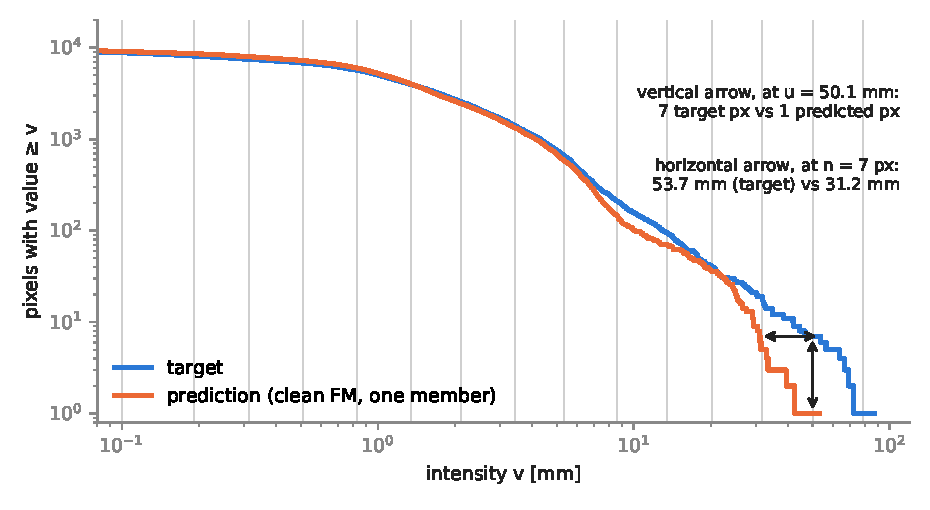
\includegraphics[width=0.9\linewidth]{figures/reward_coupling/survival.pdf}
\caption{Survival curves of a heavy validation patch (patch 979, target maximum 87\,mm) and one clean-FM member.
Vertically, at $u = 50.1$\,mm, the target has 7 pixels above the threshold and the prediction 1; the vertical term needs
a predicted pixel near 50.1\,mm to have a gradient. Horizontally, at the same count $n = 7$, the target reaches 53.7\,mm
and the prediction 31.2\,mm; this difference has a gradient on the predicted pixel of rank 7 wherever its value
is.}\label{fig:survival}
\end{figure}

\paragraph{The new area channel.} For condition $b$ and threshold $u_j$, let $n_j = \#\{i : y_i\ge u_j\}$ be the target's
count. The area entry becomes
\begin{equation}
  q_j(f) = \log\big(1 + f_{(n_j)}\big),\qquad q_j(y) = \log\big(1 + y_{(n_j)}\big),
\end{equation}
masked (weight 0) where $n_j = 0$, i.e.\ above the target maximum.

\paragraph{Its gradient.} \status{derivation} In model space $\log(1+f) = cz$, so $q_j(f) = c\,z_{(n_j)}$ and
\begin{equation}
  \frac{\partial}{\partial z_i}\big|q_j(f) - q_j(y)\big| = \pm c\quad\text{for the pixel of rank } n_j,\quad 0\ \text{otherwise.}
\end{equation}
Every populated threshold moves exactly one pixel per member, by the same amount $c$, whatever that pixel's value.
(Sorting is differentiable in the sense needed: the sorted values are a permutation of the inputs, and the gradient
flows to the selected element.) In Fig.~\ref{fig:survival} the term at $n = 7$ pushes the predicted 31.2\,mm pixel up
toward 53.7\,mm, where the vertical term gives nothing.

\paragraph{Link to Wasserstein distances, and where it breaks.} For two sets of $N$ values, the 1-D Wasserstein distance
is $W_1 = \frac1N\sum_n |f_{(n)} - y_{(n)}|$: a horizontal comparison at every rank. The same argument is made for
distributions in \citep{arjovsky2017wgan}: a horizontal (transport) distance gives a usable gradient where a vertical
comparison saturates because the supports do not overlap. Our area term is a horizontal comparison at 15 ranks only,
in log-intensity, per patch. The analogy breaks in two places: at most 15 pixels per member get a gradient, and the
comparison is per patch, not between distributions of patches.

\subsection{Inverse-mass weights for perimeter and Euler}
Perimeter and Euler stay vertical (they have no simple horizontal form) and are weighted per threshold,
\begin{equation}
  w_j = \frac{(n_j+1)^{-\alpha}}{\frac1{15}\sum_{j'}(n_{j'}+1)^{-\alpha}},\qquad \alpha = 1,
\end{equation}
so the weights average 1. Thresholds above the target maximum take the weight of the highest populated threshold, so
overshoot is penalised as strongly as the top of the target, not infinitely.

\paragraph{Why $\alpha = 1$.} \status{derivation under an assumption} The pull of threshold $u$ is the number of pixels
near it. If the survival curve is locally a power law, $S(v)\propto v^{-k}$, the pixels per unit log-intensity at $u$
are $-\mathrm dS/\mathrm d\log v = k\,S(u)\propto n_j$, and weighting by $1/n_j$ cancels it. The assumption fails where
the curve bends (the flat top below 1\,mm in Fig.~\ref{fig:survival}), so $\alpha\in\{0,0.5,1\}$ were also checked
directly, and $\alpha = 1$ spread the gradient most evenly.

\paragraph{Properness is kept.} \status{derivation} Ranks and weights depend only on the target. For each condition the
reward compares fixed feature vectors with a fixed weighted $L^1$ distance, so the energy score stays proper on these
features. If the weights depended on the prediction, this would fail.

\subsection{Checks}
\begin{itemize}[leftmargin=1.2em]
\item \textbf{Unit tests} (\texttt{tests/test\_reward\_form.py}, 13 pass) \status{measured}: a 17\,mm core under an
80\,mm target gets no gradient from the original form and is pulled up by the new one, in all three modes; unit weights
reproduce the original reward exactly; the rank feature, the masking and the weights behave as specified.
\item \textbf{Where the gradient lands} (\texttt{scripts/evaluate/reward\_threshold\_share.py}) \status{measured},
Fig.~\ref{fig:share}: on the heavy subset the share on pixels $\ge20$\,mm goes from 3.7\% to 40.9\% and below 1\,mm from
73\% to 16\%. With $\alpha = 0$ almost nothing changes: the area channel carried only 11\% of the gradient, while the
Euler term at 0.1\,mm alone carried 17--28\%.
\item \textbf{Coupling checks} (\texttt{diagnose\_coupling.py}, one heavy batch, fixed noise, 40 reward-only steps)
\status{measured}: distributional $-31.6\%$ (original $-28.1\%$), energy $-35.1\%$ (original $-32.5\%$), both above
their noise floors. The reward's sampling noise rises from 11.4\% to 18.9\% of its mean (distributional).
\end{itemize}

\begin{figure}[t]\centering
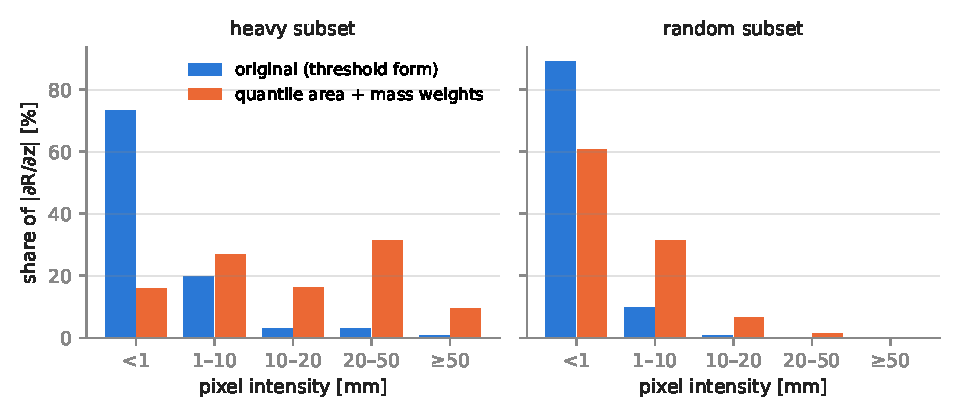
\includegraphics[width=0.95\linewidth]{figures/reward_coupling/share.pdf}
\caption{Share of the reward's model-space gradient $|\partial R/\partial z|$ on generated pixels of each intensity bin,
original form vs quantile area + mass weights ($\alpha = 1$). Clean FM, energy mode, $M=4$.}\label{fig:share}
\end{figure}

%=====================================================================
\section{Where the flow-matching loss looks}\label{sec:fmloss}
%=====================================================================

The reward is meant to correct what the base loss neglects. To know how much it must correct, we measured how the FM
loss itself spreads its gradient over intensity (\texttt{scripts/evaluate/fm\_loss\_intensity\_share.py},
\texttt{logs/fm\_loss\_intensity\_share\_v4adv.txt}; heavy subset 1,024 patches $\times$ 4 noise draws, random subset
2,048 $\times$ 2) \status{measured}.

\paragraph{How the split works.} Equation~\eqref{eq:fm} is a mean over pixels, so it splits exactly into one term per
bin $b$ of \emph{target} intensity: $\mathcal L_{\mathrm{FM}} = \sum_b L_b$ with
$L_b = \frac1N\sum_{i\in b}(v_i - u_i)^2$. For each bin we report
\begin{itemize}[nosep]
\item its share of pixels, of the loss value, and of $\sum_{i\in b}|\partial L/\partial v_i|$, the gradient on the
network's output (the analogue of $|\partial R/\partial z|$ for the reward);
\item its \emph{projection share} $\pi_b = \langle G_b, G\rangle/\|G\|^2$, with $G_b = \nabla_\theta L_b$ summed over all
batches and $G = \sum_b G_b$.
\end{itemize}
Why the projection share: a gradient step $\Delta\theta = -\eta G$ changes bin $b$'s loss, to first order, by
$\Delta L_b \approx -\eta\,\langle G_b, G\rangle$. So $\pi_b$ is the fraction of the first-order decrease of the loss that
comes from bin $b$. The $\pi_b$ sum to 1; $\pi_b < 0$ means a step along the total gradient \emph{increases} bin $b$'s
loss. (Adam rescales each parameter, so its step is not exactly $-\eta G$; $\pi_b$ is the plain-gradient version.)

\begin{figure}[t]\centering
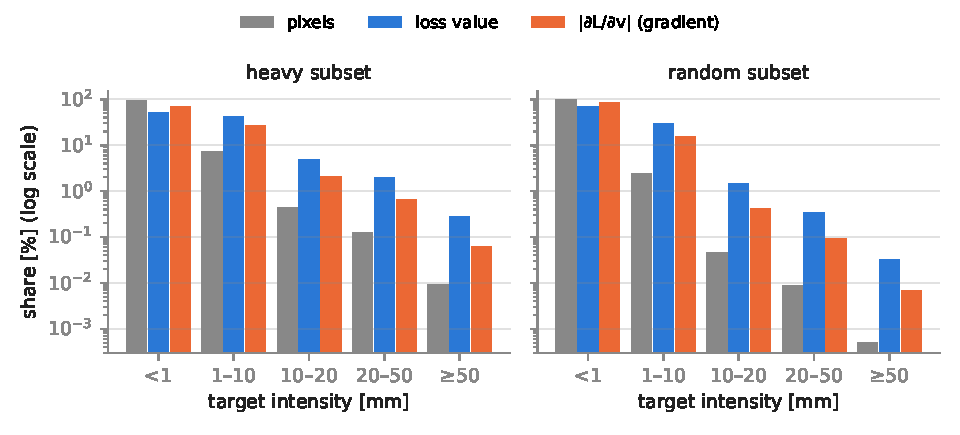
\includegraphics[width=0.95\linewidth]{figures/reward_coupling/fmloss.pdf}
\caption{Share of pixels, of the FM loss value and of its output gradient $|\partial L/\partial v|$ per target-intensity
bin, clean FM. Log scale: each grid line is a factor 10.}\label{fig:fmloss}
\end{figure}

\begin{center}\small\begin{tabular}{lccccc}\toprule
target mm & $<1$ & 1--10 & 10--20 & 20--50 & $\ge50$\\\midrule
heavy: pixels \% & 92.3 & 7.2 & 0.44 & 0.12 & 0.009\\
heavy: $|\partial L/\partial v|$ \% & 69.9 & 27.3 & 2.1 & 0.66 & 0.06\\
heavy: projection share $\pi_b$ & $+327\%$ & $-170\%$ & $-37\%$ & $-17\%$ & $-2.5\%$\\
heavy: loss per pixel (/ mean) & 0.56 & 5.8 & 11 & 16 & 30\\\midrule
random: pixels \% & 97.5 & 2.4 & 0.046 & 0.009 & 0.0005\\
random: $|\partial L/\partial v|$ \% & 84.3 & 15.2 & 0.43 & 0.09 & 0.007\\
random: projection share $\pi_b$ & $+65\%$ & $+38\%$ & $-1.9\%$ & $-1.5\%$ & $-0.2\%$\\\bottomrule
\end{tabular}\end{center}

\paragraph{Three findings.}
\begin{enumerate}[leftmargin=1.4em]
\item \textbf{Heavy rain gets about 1\% of the gradient.} Pixels $\ge20$\,mm carry 0.72\% of $|\partial L/\partial v|$ on
heavy patches and 0.10\% on random ones.
\item \textbf{It is not simply proportional to pixel count.} The squared velocity error per pixel grows with intensity
(16--30 times the mean above 20\,mm on heavy patches), so the tail's share is 5--10 times its pixel share. The model
\emph{is} worse on heavy pixels, and the loss sees it, but not enough to outweigh their rarity.
\status{withdrawn: ``any pixel-averaged loss weights an intensity level by its pixel mass'' (said in discussion on
2026-10-29). True for the sensitivity of a threshold term, not for a squared error whose size grows with intensity.}
\item \textbf{The tail pulls against the net direction.} Every bin $\ge10$\,mm has $\pi_b<0$: a plain gradient step lowers
the loss on dry pixels and raises it on heavy ones. The per-bin gradients largely cancel (on heavy patches the dry bin's
gradient alone is six times the total). Near a minimum some cancellation is expected by construction, since the total
gradient is small; the informative part is the sign. Where bulk and tail conflict, the bulk wins.
\end{enumerate}

\paragraph{Comparison with the reward.} The original reward put 3.7\% of its output gradient on pixels $\ge20$\,mm,
about five times the FM loss's 0.72\%. The comparison is rough: the reward is binned on the generated field and in $z$,
the FM loss on the target and in $v$. \status{inference, untested} This relative tilt toward the tail may be why the
distributional fine-tune moved the tail (Table~\ref{tab:fm}) even though most of its gradient was on light rain:
relative to the base loss, it was still tail-heavy.

\paragraph{Why not just reweight the FM loss? (the obvious alternative).} \status{derivation} Give each pixel a weight
$w(y)$ depending on the target. The per-pixel optimum of $\E[w(Y)(a-Y)^2\mid X]$ is
\begin{equation}
  a^\star = \frac{\E[w(Y)\,Y\mid X]}{\E[w(Y)\mid X]},
\end{equation}
a \emph{weighted} mean, no longer the conditional mean. For FM the same happens to the velocity: the sampler's output
distribution is tilted toward $p(r\mid\mathbf c)\,w$, so it would over-produce heavy rain by construction. Weighting
\emph{inside a proper score} (Section~\ref{sec:fix}) only changes how errors are traded off; the truth stays the
minimiser. This is the contrastive reason for using a feature-space reward instead of a weighted pixel loss. An
inverse-mass-weighted FM loss is still the natural baseline the reward should beat.

%=====================================================================
\section{Is the tail too noisy to learn from? (``stability in the tails'')}\label{sec:stability}
%=====================================================================

\paragraph{The question.} A whiteboard argument proposed that the reward features vary more smoothly in the tail than
the raw intensities, so they give a more \emph{stable} learning signal there. With
$F$ the cumulative distribution of pixel values, the inequality read
$\big|\partial_{F}\log P\big| > \big|\partial_{F}\log\gamma_i\big|$ for each feature $\gamma_i$. For the area channel
there are two ways to read the same tail, and the question becomes: which is more reliable, the \emph{count} reading
$\log(1+\#\{f\ge u\})$ at a fixed threshold, or the \emph{rank} reading $\log(1+f_{(n)})$ at a fixed count?

\subsection{The first-order argument}
\status{derivation} Use the tail coordinate $s = -\log(1-F)$, i.e.\ $\log$ of one over the exceedance probability.
For a generalised Pareto tail with shape $\xi$ (observed $\xi = 0.155$ on the heavy subset), the intensity at level $s$
satisfies $\log(v - u_0) \approx \xi s + \text{const}$, while the count above it is $n = N e^{-s}$. So
\begin{equation}
  \frac{\partial \log(v-u_0)}{\partial s} = \xi,\qquad \frac{\partial \log n}{\partial s} = -1 .
\end{equation}
Read literally, the whiteboard inequality \emph{fails} for the area channel whenever $\xi < 1$: the intensity changes
\emph{less} than the count per unit of tail level.

\paragraph{Noise.} An order statistic deep in the tail fluctuates by about $1/\sqrt n$ in $s$. Mapped through the slopes
above, that is $\xi/\sqrt n$ in $\log v$ and $1/\sqrt n$ in $\log n$. The rank reading is about $1/\xi$ times less noisy
in its own units. My first test, \texttt{tailstab.py}, confirmed this: independent GPD pixels, 4,000 replicate patches,
ratio of spreads 0.24--0.34.

\paragraph{But signal scales the same way.} \status{derivation} The two readings are the same survival curve read along
two axes. A model that is wrong by $\Delta s$ in tail level is wrong by $\xi\Delta s$ in the rank reading and $\Delta s$
in the count reading. Signal and noise are multiplied by the same slope, so to first order the two readings have
\emph{the same signal-to-noise ratio}. \status{withdrawn: ``the rank reading is about $1/\xi\approx6$ times more
stable'' (2026-10-29). It compared noise without signal.}

\misconception{``A feature with less noise is a better training signal.''}
{A change of variables shrinks noise and signal by the same factor. What matters is signal over noise, in the same units.}
{It is right when the signal is fixed and only the measurement is noisy, as in instrument design.}

\subsection{Beyond first order: synthetic and real tests}
\paragraph{Synthetic} (\texttt{scripts/evaluate/tail\_reading\_synthetic.py}, CPU): GPD pixels with $\xi = 0.155$, 400
conditions of 16 members each, fixed thresholds as in the reward, and a model whose intensities are scaled by $k = 0.7$
(an under-predicting model). Ratio bias/spread:

\begin{center}\small\begin{tabular}{lcccc}\toprule
& \multicolumn{2}{c}{independent pixels} & \multicolumn{2}{c}{4-px spatial correlation}\\
target count $n$ & count & rank & count & rank\\\midrule
5 & $-2.4$ & $-3.4$ & $-3.5$ & $-2.3$\\
20 & $-3.4$ & $-6.5$ & $-2.0$ & $-1.7$\\
100 & $-6.8$ & $-12.4$ & $-1.2$ & $-1.7$\\
500 & $-13.8$ & $-21.8$ & $-1.9$ & $-2.9$\\\bottomrule
\end{tabular}\end{center}

\noindent With a calibrated model ($k = 1$), both readings give a mean $|$mismatch$|$/spread of about 0.8, as expected,
so neither is biased by itself. With independent pixels the rank reading wins by 1.4--1.9 times; the reason is
nonlinear, not noise: counts collapse toward zero once the model falls short, and $\log(1+\text{count})$ has a floor at
zero. Spatial correlation makes both readings much noisier (a few correlated cells hold every extreme pixel) and the
ranking flips at $n = 5$. Masking thresholds where the target count is zero, as \texttt{quantile\_mass} does, also
creates a selection bias at small $n$ (a calibrated model looks $-1.2$ to $-1.6$ spreads low at $n=5$).

\paragraph{Real FM ensemble} (\texttt{scripts/evaluate/tail\_reading\_snr.py}, \texttt{logs/tail\_reading\_snr\_v4adv.txt};
16 members, 256 heavy and 512 random patches) \status{measured}. For every patch and threshold the target reaches, $d$ is
the member mean minus the target and $s$ the member standard deviation; the figure shows $\overline d/\mathrm{rms}(s)$
for the four features actually used by the reward, and the share of members whose maximum stays below $u$.

\begin{figure}[t]\centering
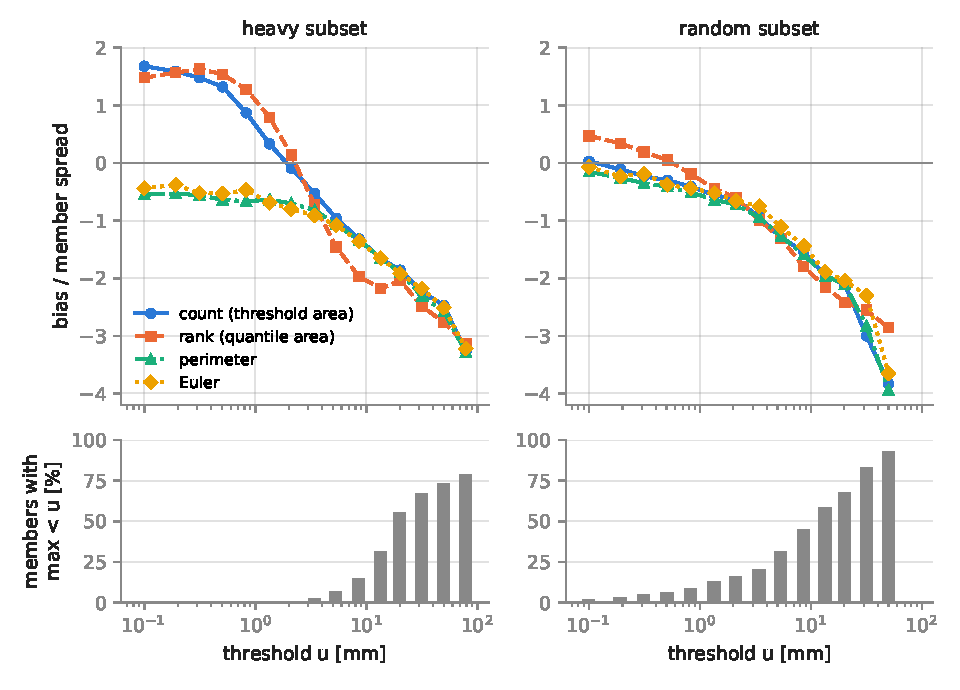
\includegraphics[width=0.95\linewidth]{figures/reward_coupling/tailsnr.pdf}
\caption{Top: systematic mismatch between the clean-FM ensemble and the target, in units of the ensemble spread, for the
two area readings, perimeter and Euler; 0 is a calibrated model. Bottom: share of members that never reach the
threshold.}\label{fig:tailsnr}
\end{figure}

\begin{enumerate}[leftmargin=1.4em]
\item \textbf{The tail deficit is visible in every feature.} Above about 5\,mm the ensemble sits 1--3 spreads below the
target, and the gap grows with $u$. Noise is not what hid the tail from the reward.
\item \textbf{The rank reading is only modestly better}: 1.1--1.5 times the count reading's bias/spread between 3 and
50\,mm, about even at 79\,mm. Perimeter and Euler track the count reading closely.
\item \textbf{Reach separates the two forms.} At 20\,mm, 55\% of members never reach the threshold; at 50\,mm, 73\% (heavy
patches). In the threshold form these members get no gradient even though their mismatch is 2--3 spreads; in the
rank form they do.
\end{enumerate}

\noindent \textbf{Conclusion of this section.} ``Stability in the tails'' does not decide between the readings. The case
for \texttt{quantile\_mass} rests on \emph{reach} and on the \emph{share of gradient} the tail receives.

%=====================================================================
\section{The general hypothesis}\label{sec:hypothesis}
%=====================================================================

The results above suggest a statement that does not depend on the Minkowski functionals.

\begin{keybox}
\textbf{Hypothesis.} A model trained on a pixel-averaged objective under-predicts heavy rain mainly because the objective
gives it a tiny share of its gradient (here $\sim$1\%) and trades it off against the bulk of the field, not mainly
because the model cannot represent it. An auxiliary objective helps the tail if
\begin{enumerate}[nosep,label=(\roman*)]
\item it puts a larger share of its gradient on high intensities than the base objective does;
\item it gives a gradient to samples that fall short of the observed tail (reach);
\item it is a proper score on the quantities it compares, so it cannot be satisfied by a wrong distribution.
\end{enumerate}
\end{keybox}

\paragraph{Why each condition is there.} (i) is Section~\ref{sec:fmloss}: the base loss leaves the tail almost unattended.
(ii) is Sections~\ref{sec:heavy} and~\ref{sec:stability}: most samples never reach the high thresholds, and a vertical
comparison is silent there. (iii) protects against the obvious way to satisfy (i) and (ii), overshooting: a reward that is
not proper can be lowered by producing too much heavy rain, or the grid-aligned filaments seen at high Study-1 weights.

\paragraph{How to test it.} Both (i) and (ii) are measurable for any candidate loss with the two new scripts:
the share of gradient per intensity bin, and the share of members out of reach. The hypothesis predicts that, at
matched total gradient norm, candidate losses rank on the tail columns as they rank on (i) and (ii). Candidates:
threshold-weighted CRPS, a pinball loss at high quantile levels, a soft FSS at high thresholds, a GPD likelihood on
exceedances, and the inverse-mass-weighted FM loss (which satisfies (i) and (ii) but not (iii)).

\paragraph{Where the hypothesis stops.} Reweighting the intensity axis can fix \emph{how much} heavy rain the model makes,
not \emph{where}. If the coarse input does not contain where the core will be, no weighting helps placement; FSS at
1\,px barely changes in any run. The assumption that would most change the conclusion is that tail error comes from
gradient allocation rather than from missing information in the input or limited capacity. The $w_{\mathrm r} = 0$
control and the comparison across candidate losses test it.

\paragraph{The ``$\eta$-learning'' note.} The whiteboard links ``other reward?'' to ``$\eta$-learning''. If $\eta_j$ means
per-threshold weights learned during training, then the $(n_j+1)^{-1}$ weights are a fixed, hand-set $\eta$. Learning
$\eta$ by \emph{minimising} the same loss collapses onto the easiest thresholds. It would need to be a min--max (the model
minimises, $\eta$ on a simplex maximises: robust over thresholds) or a constraint on the gradient share per intensity.
\status{the meaning of the term is to be confirmed by the researcher}

%=====================================================================
\section{The deterministic U-Net with the quantile form}\label{sec:unet}
%=====================================================================

The quantile form exists only in the FM reward (\texttt{reward\_finetune.py:reward\_features}). The Study-1 loss
\eqref{eq:det} still uses the threshold form, so every Study-1 run has the same pixel-mass and reach limits, and reach is
probably worse there: the vanilla backbone's exceedance ratio is 0.05--0.11 against 0.27 for FM.

\paragraph{What porting it means.} The deterministic loss has one prediction per condition, no ensemble. The quantile
area becomes a per-sample term
\[
  D_{\mathrm{area}} = \frac{1}{\xi_{15}-\xi_1}\int \mathbb 1[n_j\ge1]\,\big|\log(1+\hat f_{(n_j)}) - \log(1+y_{(n_j)})\big|\,\mathrm d\xi ,
\]
a partial, log-scale 1-D Wasserstein distance between the predicted and observed distributions of pixel values in the
patch, at 15 ranks. It needs the target \emph{field}, not only its precomputed curves, in the loss call.

\paragraph{What to expect.} \status{inference} For the backbone this term asks for the right \emph{amount} of heavy rain
per patch, wherever it is put, while the MSE penalises any core that is not in exactly the right place (the ``double
penalty''). The two terms pull against each other harder than in FM, where the reward and the FM loss act on different
things. A new weight bracket is required: the form changes the loss's gradient norm, so the \S37 weights do not carry
over.

%=====================================================================
\section{Risks, open items and the plan}\label{sec:plan}
%=====================================================================

\paragraph{Risks of the quantile form.}
\begin{itemize}[nosep,leftmargin=1.2em]
\item \textbf{Noisier reward}: 11.4\% $\to$ 18.9\% of its mean (distributional). Training-time changes are harder to see on
20 validation batches.
\item \textbf{Artefacts get more weight}: the top populated threshold may hold a handful of pixels, and the top of the
distribution contains radar artefacts. Look at the images.
\item \textbf{Sparse area gradient}: at most 15 pixels per member per step from the area term.
\item \textbf{Only proper on the features}, and blind to position.
\item \textbf{All gradient measurements are at the clean checkpoint}, before fine-tuning has moved the model.
\end{itemize}

\paragraph{Plan, in the researcher's order of priority (2026-10-30).}
\begin{enumerate}[leftmargin=1.4em]
\item \textbf{FM + Minkowski reward (distributional), quantile form.}
  \begin{enumerate}[nosep]
  \item Fix the proximal anchor so it is evaluated on the model's own coordinates (the scaled residual), with a unit
  test that the anchor is zero at initialisation and is evaluated on states the sampler visits.
  \item Re-run the coupling check with the fixed anchor.
  \item Fine-tune \texttt{config\_v4\_adv\_fm\_dist\_qm.yaml}; check the startup lines (form, weights,
  \texttt{FM\_RESIDUAL\_SCALE} source); evaluate \texttt{fm\_mink\_latest.pth} on both subsets, against the clean FM
  draws and FM + dist (threshold form). Look at the images.
  \end{enumerate}
\item \textbf{FM + Minkowski reward (energy), quantile form.}
  \begin{enumerate}[nosep]
  \item Rebalance $w_{\mathrm r}$ against $w_{\mathrm{ret}}$ by the gradient-norm rule (about $\times1000$ on
  $w_{\mathrm r}$), confirmed with \texttt{grad\_norm\_terms.py} before launching.
  \item Run the $w_{\mathrm r} = 0$ control with the same configuration, seed and budget.
  \item Fine-tune and evaluate as above.
  \end{enumerate}
\item \textbf{U-Net + Minkowski, quantile form.} Port \texttt{quantile\_mass} to the deterministic loss with tests (a
synthetic case with a known answer, and unit weights reproducing the current loss), measure its gradient share, then a
new weight bracket.
\end{enumerate}

\noindent Alongside: the fair trial of competing losses (roadmap M4) becomes the test of the general hypothesis, by
measuring (i) and (ii) for each candidate before training it.

\bibliographystyle{plainnat}
\bibliography{references_reward_coupling}
\end{document}
